\section{Exercices}

\begin{exocor}[Émission radioactive] 
	Une masse radioactive, ponctuelle, initialement neutre, située au point $O$,
	émet, à partir de l'instant $t = 0$, des particules $\alpha$ avec une vitesse
	$v_0$ supposée constante et de façon isotrope. À l'instant $t$, la charge 
	électrique située en $O$ est
	\begin{equation*}
		q(t) = q_0 \left[\exp\left(-\dfrac{t}{\tau}\right) - 1\right],
	\end{equation*}
	où $\tau$ correspond au temps de demi-vie de la masse radioactive. 
	On se place dans un repère sphérique $(O, \er, \etheta, \ephi)$. Un point
	$M$ de l'espace est repéré par ses coordonnées $(r, \theta, \phi)$. 
	On admet que le champ magnétique est nul en tout point de 
	l'espace, ce qui se démontre par des arguments de symétrie. 
	\begin{enumerate}
		\item Déterminer le champ électrique $\vece(M, t)$ 
		  en un point $M$ de l'espace pour $t > 0$.
		  Commenter.
		\item Exprimer la densité volumique de charge $\rho(M, t)$ et la
		  densité volumique de courant $\vecj(M, t)$ pour $t > 0$.
		\item Vérifier la compatibilité des résultats obtenus avec la 
		  relation locale de conservation de la charge et les équations de 
		  Maxwell.
	\end{enumerate}
\end{exocor}

\begin{exocor}[OPPH dans le vide illimité]
	\begin{enumerate}
		\item Établir l'équation de propagation du champ électrique dans 
		  le vide.
		\item Les directions de l'espace sont indiquées par la base 
		  orthonormée $(\ex, \ey, \ez)$. On envisage une solution sous 
		  forme d'onde plane progressive harmonique polarisée rectilignement
		  \begin{equation*}
			  \vece(z, t) = E_0 \cos(\omega t - k z)\ex,
		  \end{equation*}
		  où $E_0$ est l'amplitude de l'onde, $\omega$ sa pulsation temporelle
		  et $k > 0$ la pulsation spatiale. Dans quelle direction se propage
		  l'onde électromagnétique ? Quelle est l'état de polarisation 
		  de l'onde ?
	  	\item Quelle relation doivent vérifier $k$ et $\omega$ ? Utiliser
		  l'équation de propagation de $\vece$ pour aboutir à cette relation.
	  \item Déterminer le champ magnétique $\vecb(z, t)$ associé à cette onde.
	  \item Exprimer le vecteur de Poynting $\vec{\Pi}(z, t)$. 
		  En déduire la puissance 
		  $\mathcal{P}$ (moyennée en temps) traversant une surface d'aire
		  $S$ orthogonale à la direction de propagation et orientée
		  dans le sens de la propagation.
	  \item Exprimer la densité volumique $u_\mathrm{em}(z, t)$ d'énergie 
		  électromagnétique de l'onde. Que dire des termes électrique
		  et magnétique ? Moyenner $u_\mathrm{em}$ en temps. 
		\itm Exprimer de deux manières différentes l'énergie qui passe 
		  à travers $S$ durant une durée $\dt$. En déduire
		  la vitesse $v_e$ de propagation de l'énergie.
	\end{enumerate}
\end{exocor}

\begin{exocor}[Onde électromagnétique plane progressive]
	On étudie une onde électromagnétique dans un repère cartésien 
	$(O, \ex, \ey, \ez)$ dont le champ électrique 
	s'exprime en notation complexe
	\begin{equation*}
		\complex{\vece}(x, y, z, t) = \complex{E_x}(x, y, z, t) \ex + 
		\complex{E_y}(x, y, z, t)\ey 
		\quad \mathrm{avec} \quad
		\complex{E_x}(x, y, z, t) = E_0 \exp\left\{i
			\left[\dfrac{k}{3}(2x + 2y + z) - \omega t
		\right]\right\},
	\end{equation*}
	avec $\omega$ la pulsation temporelle de l'onde et $k$ une constante.
	L'onde se propage dans le vide et sa longueur d'onde $\lambda$ 
	vaut $\lambda = \unit{700}{\nano \meter}$.
	\begin{enumerate}
		\item Calculer la fréquence de l'onde. À quel domaine du spectre 
		  électromagnétique cette onde appartient-elle ?
		\item Calculer la valeur numérique de la constante $k$.
		\item Exprimer $\complex{E_y}$ en fonction de $\complex{E_x}$.
		\item Calculer le champ magnétique $\vecb(x, y, z, t)$ 
		  associée à cette onde.
		\item Calculer la densité moyenne d'énergie électromagnétique associée
		  à cette onde ainsi que sa moyenne temporelle.
	  \item Calculer le vecteur de Poynting $\vec{\Pi}(x, y, z, t)$ 
		  de cette onde et sa moyenne
		  temporelle. Commenter.
	\end{enumerate}
\end{exocor}

\begin{exocor}[Onde dans un métal]
	À suffisamment basse fréquence, un métal est localement neutre et sa
	conductivité $\gamma$ est réelle. On peut y négliger le courant de 
	déplacement devant le courant de conduction.
	\begin{enumerate}
		\item Établir l'équation de propagation vérifiée par le champ
		 électrique dans le métal.
		\item Le métal est illimité dans l'espace. On envisage une 
		  onde dont le champ électrique s'écrit, en notation complexe, 
		  \begin{equation}
			  \complex{\vece}(z, t) = E_0 \exp[i(\omega t - \complex{k}z)]\ex,
		 \end{equation}
		 où $E_0$ est une constante réelle positive. Établir la relation
		 de dispersion en faisant intervenir une distance caractéristique 
		 $\delta$ (épaisseur de peau). Donner l'expression du champ 
		 électrique. Quelle est la signification de $\delta$ ?
	 \item Établir l'expression du champ magnétique $\complex{\vecb}$ de l'onde. 
		\item Établir l'expression du vecteur de Poynting moyenné en temps.
		\item On raisonne sur un parallélépipède d'épaisseur
		  $\dz$, d'extension $L$ selon $x$ et $\ell$ selon $y$. Déterminer
		  l'expression de la puissance $\langle \mathcal{P} \rangle$ 
		  (moyennée en temps)
		  cédée à ce volume de métal par l'onde (effet Joule).
		\item En moyenne, l'énergie contenue dans ce volume reste constante.
		  En réalisant un bilan énergétique sur le volume, vérifier 
		  la cohérence des résultats des deux questions précédentes.
	\end{enumerate}
\end{exocor}

\newpage

\section{Correction}

\begin{corrige}
	\begin{enumerate}
		\item La distribution de charge est à symétrie sphérique et 
		  ne dépend spatialement que de $r$. $\vece$ est donc de la forme
		  \begin{equation*}
			  \vece(M, t) = E(r, t)\er.
		  \end{equation*}
		  Pour déterminer le champ électrique en un point $M$ de 
		  coordonnées $(r, \theta, \phi)$, on utilise le théorème de 
		  Gauss. On choisit comme surface de Gauss $\mathcal{S}$ une sphère de 
		  rayon $r$ et de centre $O$. Le théorème de Gauss s'écrit alors
		  \begin{equation*}
			  \oiint_{P \in \mathcal{S}} \vece(P, t) \cdot \ds 
			  = \dfrac{Q(t)}{\epsilon_0},
		  \end{equation*}
		  où $Q(t)$ est la charge contenue dans $\mathcal{S}$ à l'instant
		  $t$. Pour cette surface, $\ds = r^2 \sin \theta \dtheta \dphi \er$.
		  Le membre de gauche s'écrit donc
		  \begin{equation*}
			  \oiint_{P \in \mathrm{S}} \vece(P, t) \cdot \ds =
			  4 \pi r^2 E(r, t).
		  \end{equation*}
		  Pour déterminer le membre de droite, il est nécessaire d'exprimer
		  la charge $Q$ contenue dans la sphère à l'instant $t$. On a
		  alors deux cas de figure
		  \begin{enumerate}
			  \item si $t < \dfrac{r}{v_0}$, aucune charge n'est 
			    sortie de la sphère. On a donc $Q = 0$,
			  \item si $t \ge \dfrac{r}{v_0}$, toutes les charges
		            qui ont été émises à un temps antérieur à $t -
			    \dfrac{r}{v_0}$ ont eu le temps de sortir de la sphère.
			    On a donc
			    \begin{equation*}
				    Q(t) = q\left(t - \dfrac{r}{v_0} \right)
				      = q_0 \left[\exp\left(- \dfrac{t - 
					      \dfrac{r}{v_0}}{\tau}\right) - 1
					   \right].
			   \end{equation*}
		  \end{enumerate}
		  Finalement, on aboutit à l'expression de $\vece(M, t)$
		  \begin{equation*}
			  \boxed{
			  \vece(r, t) =
			  \left\{
			  \begin{array}{l}
				  \vec{0} \quad \mathrm{si} \quad t < 
				  \dfrac{r}{v_0} \\[1em]
				  \dfrac{q_0}{4 \pi \epsilon_0 r^2}
				  \left[\exp\left(- \dfrac{t - 
			          \dfrac{r}{v_0}}{\tau}\right) - 1 \right]\er
				  \quad \mathrm{si} \quad t \ge \dfrac{r}{v_0}.
		         \end{array}
			 \right.
		 }
		\end{equation*}

	\item Pour déterminer $\rho(r, t)$, on exprime la charge $\delta Q(t)$ contenue
	  entre les sphères de rayon $r$ et de rayon $r + \dr$ à l'instant 
	  $t > \dfrac{r}{v_0}$ de deux manières
	  \begin{enumerate}
		  \item $\delta Q(t) = Q(r + \dr, t) - Q(r, t) = \dd{Q}{r}(r, t) \dr
		  = \dfrac{q_0}{v_0 \tau} \exp\left(-\dfrac{t - \dfrac{r}{v_0}}
		  {\tau}\right) \dr$
	  	  \item $\delta Q(t) = 4 \pi r^2 \dr \rho(r, t)$.
	  \end{enumerate}
	  En égalant les deux expressions, on obtient
	  \begin{equation*}
		  \boxed{
		  \rho(r, t) = \dfrac{q_0}{4 \pi r^2 v_0 \tau}
		  \exp\left(-\dfrac{t - \dfrac{r}{v_0}} {\tau}\right).
	  }
	  \end{equation*}
	  On en déduit le vecteur densité de courant $\vecj$
	  \begin{equation*}
		  \boxed{
		  \vecj(r, t) = \rho(r, t) v_0 \er  = \dfrac{q_0}{4 \pi r^2 \tau}
		  \exp\left(-\dfrac{t - \dfrac{r}{v_0}} {\tau}\right) \er.
	  }
  	  \end{equation*}

  	\item On vérifie dans un premier temps l'équation de conservation de 
	  la charge. Il est nécessaire pour cela de calculer la dérivée temporelle
	  de $\rho$ et la divergence de $\vecj$. Pour la dérivée temporelle, 
	  on a directement
	  \begin{equation*}
		  \dd{\rho}{t}(r, t) = - \dfrac{\rho(r, t)}{\tau}.
	  \end{equation*}
	  La divergence de $\vecj$ donne
	  \begin{equation*}
		  \div \vecj(r, t) = \dfrac{\rho(r, t)}{\tau}.
	  \end{equation*}
	  L'équation de conservation de la charge est vérifiée. On peut alors
	  s'intéresser à l'équation de Maxwell-Ampère
	  \begin{equation*}
		  \vec{0} = \vecj(r, t) + \epsilon_0 \dd{\vece}{t}(r, t).
	  \end{equation*}
	  La dérivée temporelle de $\vece$ donne directement
	  \begin{equation*}
		  \dd{\vece}{t} = - \dfrac{\vece}{\tau} = - \dfrac{\vecj}{\epsilon_0}.
	  \end{equation*}
	  L'équation de Maxwell-Ampère est bien vérifiée.
	\end{enumerate}
\end{corrige}

\begin{corrige}
	\begin{enumerate}
		\item Pour déterminer l'équation de propagation du champ électrique
		  dans le vide, on commence par écrire le rotationnel de 
		  l'équation de Maxwell-Faraday
		  \begin{equation*}
			  \rot[\rot \vece(M, t)] = -\rot\left[\dd{\vecb}{t}(M, t)\right].
		  \end{equation*}
		  \begin{itemize}
		 	 \item On s'intéresse dans un premier temps au membre 
			   de droite de cette équation. Il est tout à fait possible 
			   de faire commuter les dérivées spatiale et temporelle ici.
			   On peut ensuite se servir de l'équation de Maxwell-Ampère
			   dans le vide pour exprimer le rotationnel de $\vecb$
			   \begin{equation*}
				   \rot \vecb(M, t) = \mu_0 \epsilon_0 
				   \dd{\vece}{t}(M, t).
			   \end{equation*}
			   Le membre de droite devient donc
			   \begin{equation*}
				   - \rot\left[\dd{\vecb}{t}(M, t)\right] = 
				   - \mu_0 \epsilon_0 \dd{^2\vece}{t^2}(M, t).
			  \end{equation*}

		  	\item Pour le membre de gauche, on se souvient de l'égalité
			  vectorielle
			  \begin{equation*}
				  \rot[\rot \vece] = \grad(\div \vece) - 
				  \laplacien \vece,
			  \end{equation*}
			  où $\laplacien$ est le laplacien vectoriel. Or d'après
			  l'équation de Maxwell-Gauss dans le vide ($\rho = 0$)
			  \begin{equation*}
				  \div \vece = 0.
			  \end{equation*}
			  Finalement, le membre de gauche s'écrit
			  \begin{equation*}
				  \rot(\rot \vece) = -\laplacien \vece.
			  \end{equation*}
		  \end{itemize}
		  On retrouve donc bien l'équation de propagation du champ électrique
		  dans le vide
		  \begin{equation*}
			  \boxed{
				  \laplacien \vece(M, t) - \mu_0 \epsilon_0
				  \dd{^2 \vece}{t^2}(M, t) = \vec{0},
		  }
		  \end{equation*}
		  où $c = \dfrac{1}{\sqrt{\epsilon_0 \mu_0}}$ est la vitesse
		  de propagation de la lumière dans le vide.

	  \item L'onde se propage selon \fbox{l'axe $(Oz)$ vers les $z$ croissants.}
	    Le champ électrique est dirigé selon $\ex$, \fbox{la polarisation de l'onde
    	    est donc selon $\ex$.}

	  \item On injecte l'OPPH dans l'équation de propagation de $\vece$ 
	    déterminée plus haut. Il faut donc calculer le laplacien et 
	    la dérivée seconde de $\vece$
	    \begin{description}
		    \item[Laplacien : ] Pour le laplacien on a
		    \begin{equation*}
			\laplacien \vece = \dd{^2}{z^2}[E_0 \cos(\omega t - k z)]
			= - E_0 k^2 \cos(\omega t - k z).
		    \end{equation*}

	    	\item[Dérivée seconde par rapport au temps : ] De la même manière, 
		 on peut calculer la dérivée seconde de $\vece$ par rapport au temps
		 \begin{equation*}
			 \dd{^2\vece}{t^2} = - \omega^2 E_0 \cos(\omega t - k z)\ex.
	         \end{equation*}
	    \end{description}
	    L'équation de propagation devient alors
	    \begin{equation*}
		    \left[k^2 - \left(\dfrac{\omega}{c}\right)^2\right]
		    E_0 \cos(\omega t - k z) = 0.
	    \end{equation*}
	    Cette équation doit être vérifiée en tout $z$ et en tout $t$ ! Il est 
	    donc indispensable que
	    \begin{equation*}
		    \boxed{
			    k = \dfrac{\omega}{c}.
			  }
	    \end{equation*}

    	   \item Pour déterminer l'expression du champ magnétique $\vecb$, on utilise
      	     l'équation de Maxwell-Faraday
      	     \begin{equation*}
		     \rot \vece(M, t) = - \dd{\vecb}{t}(M, t).
	     \end{equation*}
	     Le rotationnel de $\vece$ se calcule directement
	     \begin{equation*}
		     \rot \vece(M, t) = \dd{}{z} [E_0\cos(\omega t - k z)] \ey
		 	    = E_0 k \sin(\omega t - k z) \ey.
	     \end{equation*}
	     On en déduit
	     \begin{equation*}
		     \boxed{
			     \vecb(M, t) = \dfrac{E_0}{c} \cos(\omega t - k z) \ey.
			   }
	     \end{equation*}

     \item Le vecteur de Poynting $\vec{\Pi}$ est donné par
	  \begin{equation*}
		  \vec{\Pi}(M, t) = \dfrac{\vece(M, t) \wedge \vecb(M, t)}{\mu_0}
		  = \dfrac{E_0^2 \cos^2(\omega t - k z)}{\mu_0 c} \ez
		  = \boxed{\epsilon_0 c E_0^2 \cos^2(\omega t - kz) \ez},
	  \end{equation*}
	  car $c^2 = \dfrac{1}{\mu_0 \epsilon_0}$.
     \item La puissance moyennée en temps traversant une surface d’aire $S$ est
	   donnée par
	   \begin{equation*}
		   \boxed{
			   \mathcal{P} = \langle \Pi(M,t) \rangle S = 
		   c \epsilon_0 E_0^2
		   \dfrac{1}{T} \int_{t = 0}^{t = T} \cos^2(\omega t - kz) \dt
		   = \dfrac{\epsilon_0 c E_0^2}{2}S,
	   }
	   \end{equation*}
	   où $\langle \rangle$ correspond à une moyenne temporelle et où $T$ 
	   est la période de l'onde.

     \item La densité volumique d'énergie s'exprime
	   \begin{equation*}
		   u_\mathrm{em}(z, t) = \dfrac{\epsilon_0 E^2(z, t)}{2} + 
		   \dfrac{B^2(z, t)}{2 \mu_0}.
	   \end{equation*}
	   Or, $B = E/c$ et $\mu_0 \epsilon_0 c^2 = 1$, on obtient donc
	   \begin{equation*}
		   \boxed{
			   u_\mathrm{em}(z, t) = \epsilon_0 E_0^2 \cos^2(\omega t - kz)
	   }.
   	\end{equation*}
	On remarque que les contributions électrique et magnétique à la densité 
	volumique d'énergie électromagnétique \fbox{sont égales}. La densité
	volumique d'énergie électromagnétique moyennée en temps est donnée par
	\begin{equation*}
		\fbox{
		\langle u_\mathrm{em} \rangle = \dfrac{\epsilon_0 E_0^2}{2}
		.}
	\end{equation*}
	\item On note $v_e$ la vitesse de propagation de l'énergie. L'énergie 
	      traversant la surface $S$ durant un instant $\dt$ s'exprime de deux
	      manières équivalentes
	      \begin{enumerate}
		      \item Il s'agit de la quantité d'énergie $\delta U$ contenue dans 
			    un cylindre de section $S$ et de longueur 
			    $\dz = v_e \dt$ (voir Fig.~\ref{fig:maxwell_bilan_ex})
			    \begin{equation*}
				    \delta U = v_e \dt \iint_S \langle
				    u_\mathrm{em} \rangle \dx \dy =
				    \dfrac{\epsilon_0 E_0^2}{2} S v_e \dt.
			   \end{equation*}
		     \item C'est la puissance rayonnée à travers la section $S$
			   multiplié par $\dt$
			   \begin{equation*}
				   \delta U = \langle \Pi \rangle S \dt = 
				   \dfrac{E_0^2 S}{2 \mu_0 c} \dt.
			  \end{equation*}

			  En identifiant les deux expressions précédentes de 
			  $\delta U$, on trouve 
			  \begin{equation*}
				  \boxed{
				  v_e = c.
			  }
			  \end{equation*}
	     \end{enumerate}
	\end{enumerate}
	\begin{figure}[htpb]
		\centering
		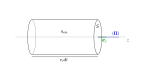
\includegraphics[scale=0.8]{bilan_exercice}
		\caption{L'énergie qui traverse la section $S$ durant une durée
		$\dt$ est contenue dans un cylindre de section $S$ et de 
		longueur $v_e \dt$.}%
		\label{fig:maxwell_bilan_ex}
	\end{figure}
	\begin{defn}[Vitesse d'avancée de l'énergie pour une OPPM]
		Pour une OPPM dans le vide illimité, l'énergie se déplace 
		à la vitesse de la lumière. Attention, ce n'est pas forcément le
		cas si l'onde n'est pas une OPPH.
	\end{defn}
\end{corrige}

\begin{corrige}
\begin{enumerate}
	\item Le vecteur d'onde s'exprime $\mathbf{k} = \dfrac{k}{2}
		(2 \ex + 2\ey + \ez)$ et sa norme vaut $k$. $k$ est relié à 
	      $\lambda$ par la relation $k = \dfrac{2 \pi}{\lambda}$. Or la relation 
	      de dispersion permet de relier la pulsation temporelle $\omega$
	      à la pulsation spatiale $k$ 
	      \begin{equation*}
		      k = \dfrac{\omega}{c}.
	      \end{equation*}
	      On obtient finalement
	      \begin{equation*}
		      f = \dfrac{\omega}{2 \pi} = \dfrac{k c}{2 \pi} 
		      = \dfrac{c}{\lambda} = \boxed{\unit{4.2 \times 10^{14}}{\hertz}.}
	      \end{equation*}
	      Cette onde appartient au \fbox{domaine du visible}.
	\item On calcule directement la valeur de $k$ 
	      \begin{equation*}
		      \boxed{
		      k = \dfrac{2 \pi}{\lambda} = \unit{9.0 \times 10^6}{\rad 
		      \usk \rp \meter}.
	      }
      	      \end{equation*}
	\item L'onde électromagnétique se déplace dans le vide, l'équation de 
	     Maxwell-Gauss devient alors
	     \begin{equation*}
		     \div \complex{\vece} = 0.
	     \end{equation*}
	     On a alors
	     \begin{equation*}
		     \dd{\complex{E_x}}{x} + \dd{\complex{E_y}}{y} = 0 \Rightarrow 
		     \dd{\complex{E_y}}{y} = -i \dfrac{2 k}{3} \complex{E_x}
		     \Rightarrow \boxed{\complex{E_y} = -\complex{E_x}.}
	    \end{equation*}

	\item L'onde étant une OPPH, on peut utiliser l'équation de Maxwell-Faraday
	      en notation complexe
	      \begin{equation*}
		      \complex{\vecb} = \dfrac{\vec{k} \wedge \complex{\vece}}{w} = \quad
		      \vline
		      \begin{array}{r}
			      \dfrac{2k}{3} \\[1em]
			      \dfrac{2k}{3} \\[1em]
			      \dfrac{k}{3}
		      \end{array}
		      \wedge \quad 
		      \vline
		      \begin{array}{l}
			      \complex{E_x} \\[1em]
			      -\complex{E_x} \\[1em]
			      0 
		      \end{array}
		      = \boxed{\dfrac{\complex{E_x}}{3c}(\ex + \ey - 4\ez).}
	     \end{equation*}
	\item Pour déterminer la densité volumique d'énergie électromagnétique
	      $u_\mathrm{em}$, il est nécessaire d'utiliser les expressions
	      réelles $\vece$ et $\vecb$ des champs électrique et magnétique. 
	      On les obtient en prenant les parties réelles de $\complex{\vece}$
	      et $\complex{\vecb}$
	      \begin{equation*}
		      \vece(x, y, z, t) = E_0 \cos\left[
		      \dfrac{k}{3}(2x + 2y +z) - \omega t \right](\ex - \ey)
	      \end{equation*}
	      et
	      \begin{equation*}
		      \vecb(x, y, z, t) = \dfrac{E_0}{3c} \cos\left[
		      \dfrac{k}{3}(2x + 2y +z) - \omega t \right](\ex + \ey - 4\ez)
	      \end{equation*}
	      On peut alors déterminer l'expression de $u_\mathrm{em}$
	      \begin{equation*}
		      \begin{array}{rcl}
			      u_\mathrm{em}(x, y, z, t) &=& 
			\dfrac{\epsilon_0 E^2(x, y, z, t)}{2} 
			+ \dfrac{B^2(x, y, z, t)}{2 \mu_0} \\[1em]
			   &=& \dfrac{\epsilon_0 E_0^2}{2} \cos^2\left[
		      \dfrac{k}{3}(2x + 2y +z) - \omega t \right] \times 2 +
		      \dfrac{E_0^2}{18 \mu_0 c^2} \cos^2\left[
		      \dfrac{k}{3}(2x + 2y +z) - \omega t \right] \times 18 \\[1em]
		      	  &=& \epsilon_0 E_0^2 \cos^2\left[
		      \dfrac{k}{3}(2x + 2y +z) - \omega t \right] +
		      \espilon_0 E_0 ^2 \cos^2\left[
		      \dfrac{k}{3}(2x + 2y +z) - \omega t \right]\\[1em]
			  &=& 2 \epsilon_0 E_x^2(x, y, z, t)
		      \end{array}
	      \end{equation*}
	      \begin{equation*}
		      \boxed{
		      \langle u_\mathrm{em} \rangle = \epsilon_0 \vece_0^2
	      }
      	     \end{equation*}

	\item Le vecteur de Poynting $\vec{\Pi}$ est donné par 
	      \begin{equation*}
		      \begin{array}{rcl}
			      \vec{\Pi(x, y, z, t)} &=& \dfrac{\vece \wedge \vecb}
			      {\mu_0} \\[1.2em]
		      	      &=& \dfrac{E_x^2(x, y, z, t)}{3\mu_0c} \left(
			      \quad \vline
			      \begin{array}{c}
				      1 \\
				      - 1 \\
				      0
			      \end{array}
			      \wedge \quad
			      \vline
			      \begin{array}{c}
				      1 \\
				      1 \\
				      -4
			      \end{array}
		      \right) \\[1.2em] 
			&=& \dfrac{c \epsilon_0 E_x^2(x, y, z, t)}
			{3}(4\ex + 4\ey + 2\ez) \\[1em]
			&=& \dfrac{2 c \epsilon_0 E_x^2(x, y, z, t)}
			{3}(2\ex + 2\ey + \ez)
	      \end{array}
	      \end{equation*}
	      Finalement, on calcule la moyenne du vecteur de Poynting
	      \begin{equation*}
		      \boxed{
		      \langle \vec{\Pi} \rangle = 
		      \dfrac{c \epsilon_0 E_0^2}{3}(2\ex + 2\ey + \ez).
	      }
      	      \end{equation*}
	      On remarque que la norme de ce vecteur vaut
	      \begin{equation*}
		      \langle \Pi \rangle = \dfrac{c \epsilon_0 E_0^2}{3} \times 3
		      = c \epsilon_0 E_0^2 = c \langle u_\mathrm{em} \rangle.
	      \end{equation*}
	      Cette relation traduit le fait que l'énergie se déplace à la vitesse
	      $c$ dans le vide pour une OPPH.
\end{enumerate}
\end{corrige}

\begin{corrige}
	\begin{enumerate}
		\item Le champ électrique $\vece$ est relié au vecteur densité de courant
		$\vecj$ par la loi d'Ohm locale dans les conducteurs
		\begin{equation*}
			\vecj = \gamma \vece.
		\end{equation*}
		Le métal étant localement neutre, la densité volumique de charge
		$\rho$ est nulle. Les champs électrique $\vece$ et magnétique $\vecb$
		vérifient les équations de Maxwell suivantes 

		\begin{description}[labelindent=2em, itemsep=1em]
			\item[Maxwell-Gauss : ] $\div \vece = 0$,
			\item[Maxwell-Faraday : ] $\rot \vece = -\dd{\vecb}{t}$,
			\item[Maxwell-Thomson : ] $\div \vecb = 0$,
			\item[Maxwell-Ampère : ] $\rot \vecb = \mu_0 \gamma \vece$.
		\end{description}
		Comme d'habitude, il suffit ensuite de prendre le rotationnel
		de l'équation de Maxwell-Faraday
		\begin{equation*}
			\rot(\rot \vece) = -\rot\left(\dd{\vecb}{t}\right).
		\end{equation*}
		Le terme de droite devient grâce à l'équation de Maxwell-Ampère
		\begin{equation*}
			-\rot\left(\dd{\vecb}{t}\right) = -\mu_0 \gamma \dd{\vece}{t}.
		\end{equation*}
		Le terme de gauche devient grâce à l'équation de Maxwell-Gauss
		\begin{equation*}
			\rot(\rot \vece) = \grad(\div \vece) - \laplacien \vece
			= -\laplacien \vece.
		\end{equation*}
		Finalement, on aboutit à l'équation de diffusion du champ électrique
		dans le métal
		\begin{equation*}
			\boxed{
			\dd{\vece}{t} = \dfrac{1}{\mu_0 \gamma}\laplacien \vece.
		}
		\end{equation*}
	\item On injecte la forme d'onde proposée par l'énoncé dans l'équation
	      de diffusion, on obtient alors la relation de dispersion
	      \begin{equation*}
		      i \omega \complex{\vece} = \dfrac{(-i\complex{k})^2}{\gama \mu_0}
		      \complex{\vece} \Rightarrow \boxed{\complex{k}^2 = -i \mu_0 \gamma 
		      \omega.}
	      \end{equation*}
	      Pour déterminer $\complex{k}$, on cherche alors la racine carrée de 
	      $i$. Pour ce faire, on écrit
	      \begin{equation*}
		      i = \exp\left[i\left(\dfrac{\pi}{2} + 2 k \pi \right)\right]
		      \quad \mathrm{avec} \quad k \in \mathbb{Z}.
	      \end{equation*}
	      On en déduit l'expression de $\complex{k}$
	      \begin{equation*}
		      \complex{k} = \sqrt{\mu_0 \gamma}\exp
		      \left[i\left(\dfrac{\pi}{4} +  k \pi \right)\right]
		      \quad \mathrm{avec} \quad k \in \mathbb{Z}.
	     \end{equation*}
	     Cette expression se simplifie en 
	     \begin{equation*}
		     \boxed{
		     \complex{k} = \pm \dfrac{1 - i}{\delta},
		     \quad \mathrm{avec} \quad \delta = \sqrt{\dfrac{2}{\mu_0 \gamma
		     \omega}}
	     .}
     	     \end{equation*}
	     Il y a donc deux solutions possibles. On choisit ici de retenir la
	     solution avec le signe $-$. Le champ électrique sous forme complexe
	     s'écrit alors
	     \begin{equation*}
		     \boxed{
			     \complex{\vece(z, t)} = E_0 \exp\left(\dfrac{-z}{\delta}
				     \right)\exp\left[i\left(\omega t - 
				     \dfrac{z}{\delta}\right)\right]\ex
		     }
	     \end{equation*}
	     En notation réelle, il devient
	     \begin{equation*}
		     \vece(z, t) = E_0 \exp\left(\dfrac{-z}{\delta}
				     \right)\cos\left(\omega t - 
				     \dfrac{z}{\delta}\right)\ex
	     \end{equation*}
	     L'onde se propage selon la direction $\ez$ mais son amplitude s'amortit
	     au cours de la propagation. $\delta$ représente donc la longueur
	     caractéristique sur laquelle le champ s'atténue.
     	\item La propagation de l'onde électrique est décrite par une 
	      pseudo-OPPH (le pseudo étant dû à la nature complexe
	      de $\complex{\vec{k}}$). À part la nature complexe du vecteur
	      d'onde, $\complex{\vece}$ a la même forme que dans le cas d'une
	      OPPH. L'équation de Maxwell-Ampère peut donc toujours s'écrire 
	      sous la forme
	      \begin{equation*}
		      \complex{\vecb(z, t)} = \dfrac{\complex{\vec{k}} \wedge 
		      \complex{\vece(z, t)}}{\omega},
	      \end{equation*}
	      où $\complex{\vecb}$ est le champ magnétique.
      Comme $\complex{\vec{k}} = \complex{k} \ez$, on a directement
	      \begin{equation*}
		      \boxed{
			      \complex{\vecb(z, t)} = E_0 \dfrac{1 - i}{\delta \omega}
		      \exp\left(- \dfrac{z}{\delta}\right)
		      \exp\left[i\left(\omega t - \dfrac{z}{\delta}\right)\right] \ey.
	      }
      	      \end{equation*}
	      On réécrit $1 - i$ sous forme exponentielle, cela donne
	      \begin{equation*}
		      1 - i = \sqrt{2} \exp\left(-i\dfrac{\pi}{4}\right).
	      \end{equation*}
	      $\complex{\vecb}$ peut alors se mettre sous la forme d'une exponentielle
	      \begin{equation*}
		      \complex{\vecb(z, t)} = \dfrac{\sqrt{2}E_0}{\delta \omega}
		      \exp\left(- \dfrac{z}{\delta}\right)
		      \exp\left[i\left(\omega t - \dfrac{z}{\delta} - \dfrac{\pi}{4}
		      \right)\right] \ey.
	      \end{equation*}
	      Sous une forme réelle, cela donne
	      \begin{equation*}
		      \vecb(z, t) = \dfrac{\sqrt{2}E_0}{\delta \omega}
		      \exp\left(- \dfrac{z}{\delta}\right)
		      \cos\left(\omega t - \dfrac{z}{\delta} - \dfrac{\pi}{4}
		      \right) \ey.
	      \end{equation*}
	      électrique.
      \item Le vecteur de Poynting $\vec{\Pi}$ est défini par 
	    \begin{equation*}
		    \boxed{
			    \vec{\Pi}(z, t) = \dfrac{\vece(z,t) \wedge 
			    \vecb(z, t)}{\mu_0}
		            = \dfrac{\sqrt{2} E_0^2}{\delta \omega \mu_0}
			    \exp\left(-\dfrac{2z}{\delta}\right)
			      \cos\left(\omega t - \dfrac{z}{\delta}\right)
			      \cos\left(\omega t - \dfrac{z}{\delta} 
			      - \dfrac{\pi}{4} \right) \ez.
			  }
	   \end{equation*}
	   Or, en développant le second $\cos$ on obtient
	   \begin{equation*}
		   \cos\left(\omega t - \dfrac{z}{\delta} - \dfrac{\pi}{4}\right) = 
			\cos\left(\omega t - \dfrac{z}{\delta}\right) 
			\cos\left(\dfrac{\pi}{4}\right) + 
			\sin\left(\omega t - \dfrac{z}{\delta}\right) 
			\sin\left(\dfrac{\pi}{4}\right) =
			\dfrac{\cos\left(\omega t - \dfrac{z}{\delta}\right)
			+ \sin\left(\omega t - \dfrac{z}{\delta}\right)}
			{\sqrt{2}}
	   \end{equation*}
	   Calculer la moyenne de $\vec{\Pi}$ va revenir à calculer l'intégrale
	   d'un $\cos^2$ et d'un $\cos$ multiplié par un $\sin$ sur une
	   période temporelle. La moyenne du produit des deux fonctions trigonométriques
	   donne $0$ tandis que la moyenne de $\cos^2$ donne $1/2$. Finalement, 
	   on aboutit à l'expression de la moyenne temporelle $\langle \vec{\Pi} \rangle$
	   du vecteur de Poynting
	   \begin{equation*}
		   \boxed{
			   \langle \vec{\Pi} \rangle(z) = \dfrac{E_0^2}{2 
			   \mu_0 \delta \omega}
		   	   \exp\left(-\dfrac{2z}{\delta}\right) \ez .
	   }
   	   \end{equation*}
	   On remarque que contrairement aux exercices précédents $\langle 
	   \vec{\Pi} \rangle$ dépend de $z$.
	   \item La puissance cédée par unité de volume et par effet Joule au métal
		 s'écrit $\mathcal{P}_\mathrm{J} = \vecj \cdot \vece$. Or, 
		 d'après la loi d'Ohm locale $\vecj = \gamma \vece$ donc
		 \begin{equation*}
			 \boxed{
				 \mathcal{P}_\mathrm{J}(z,t) = \gamma \vece^2(z,t)
			 = \gamma E_0^2 \exp\left(-\dfrac{2z}{\delta}\right)
			   \cos^2\left(\omega t - \dfrac{z}{\delta}\right).
		   }
	 	 \end{equation*}
		 Moyenner $\mathcal{P}_\mathrm{J}$ en temps revient à moyenner
		 un $\cos^2$ en temps, on aboutit donc à l'expression de la 
		 moyenne temporelle de $\mathcal{P}_\mathrm{J}$
		 \begin{equation*}
			 \boxed{
				 \langle \mathcal{P}_\mathrm{J} \rangle(z) = 
				\dfrac{\gamma E_0^2}{2}\exp
				\left(-\dfrac{2z}{\delta}\right)
			}
		\end{equation*}
		Pour déterminer $\langle \mathcal{P} \rangle$, il faut alors intégrer 
		$\langle \mathcal{P}_\mathrm{J} \rangle$ sur le volume. 
		$\langle \mathcal{P}_\mathrm{J} \rangle$ ne dépend ni de $x$
		ni de $y$ et la dimension $\dz$ du volume est infinitésimale, 
		on a donc
		\begin{equation*}
			\boxed{
				\langle \mathcal{P} \rangle = $\langle 
				\mathcal{P}_\mathrm{J} \rangle$
				L \ell \dz
				=\dfrac{\gamma E_0^2}{2} 
		      \exp\left(-\dfrac{2z}{\delta}\right) L \ell \dz.
		}
		\end{equation*}

	\item On réalise un bilan énergétique sur le volume. On note $\phi(z)$
	      le flux d'énergie entrant dans le volume et $\phi(z + \dz)$ le
	      flux d'énergie sortant du volume. En moyenne, l'énergie contenue
	      dans le volume se conserve, on a donc
	      \begin{equation*}
		      \phi(z) = \phi(z + \dz) + \langle \mathcal{P} \rangle.
	      \end{equation*}
	      On a donc
	      \begin{equation*}
		      \boxed{
		      -\dn{\phi}{z}(z) = \dfrac{\gamma E_0^2}{2} 
		      \exp\left(-\dfrac{2z}{\delta}\right) L \ell.
	      }
      	      \end{equation*}
	      Or, $\phi(z)$ s'obtient en intégrant la moyenne du vecteur de 
	      Poynting sur une section du volume
	      \begin{equation*}
		      \phi(z) = \langle \Pi \rangle L \ell = 
		      	   \dfrac{E_0^2}{2 \mu_0 \delta \omega} \exp\left(
			    - \dfrac{2z}{\delta}\right) L \ell.
	      \end{equation*}
	      On a donc en dérivant et en remplaçant $\delta$ par son expression
	      \begin{equation*}
		      \boxed{
		      \dn{\phi}{z} = -\dfrac{E_0^2}{\mu_0 \delta^2 \omega}
		      \exp\left(-\dfrac{2z}{\delta}\right)L \ell=
		      - \dfrac{\gamma E_0^2}{2} \exp\left(-\dfrac{2z}{\delta} L \ell
			      \right).
		      }
	     \end{equation*}
	     On retrouve bien la bonne expression.
\end{enumerate}
\end{corrige}
